\section{Implementation}
As evaluated in the last section we will proceed to implement TF-DAC-MACS with small adaptions for a practical secure cloud storage system. To do so we need to implement five entities:  

\begin{itemize}
	\item \textbf{The Server} will do the inital setup of the public paramter used in the later process. It will publish this information on a public bulliton board. Further, it will trigger and permit AA creations. The server will create a \textit{Authority Identifier} (\ac{AID}) that is unique in this system. The server is assumed to be honest-but-curious.
	\item \textbf{Certificate Authority (\ac{CA})} issues a certificate for the GID of the user. This certificate can be revoced so that the user is not able to optain new secret keys from the AA oder other data owners. The CA is fully trusted.
	\item \textbf{Attribute Authority (\ac{AA})} creates the secret keys for its attributes. Attributes are prefixed with the \ac{AID} to ensure uniqueness among the attribute universe. AA are also trusted but never collude with users.
	\item \textbf{Data owner} Data owner can issue two-factor keys to trusted user. Only users owning a secret authentication key can decipher the a given cipher text if it is secured with the previous exchanged two-factor key (\ac{2FA}-Key). User are untrusted.
	\item \textbf{Cloud storage provider (\ac{CSP})} The cloud storage provider provide storage to save the encrypted files.
	\item \textbf{Users} Users download and decipher ciphertext. They receive attribute secret keys from the AA, GID and certifidates from the server and two factor keys from the data owners. The CSP is honest-but-curious as well.
\end{itemize}

In the following sections, the differene phases Setup, encrypt, decrypt, attribute revocation and authentication key revocation are shortly explained.

For en- and decryption we will still use the process of encyrpting the file symetrically to create a file key which will then encrypted under the attribute policy. This reduces the size of the content that will be encrypted with ABE to a minimum. Moreover, we can still benefit from the great performance of \ac{AES}. Please note that for any scheme details we referre to the paper of TF-DAC-MACS \cite{li2017two}.

\subsection{Setup}
\begin{figure}[!ht]
\centering
    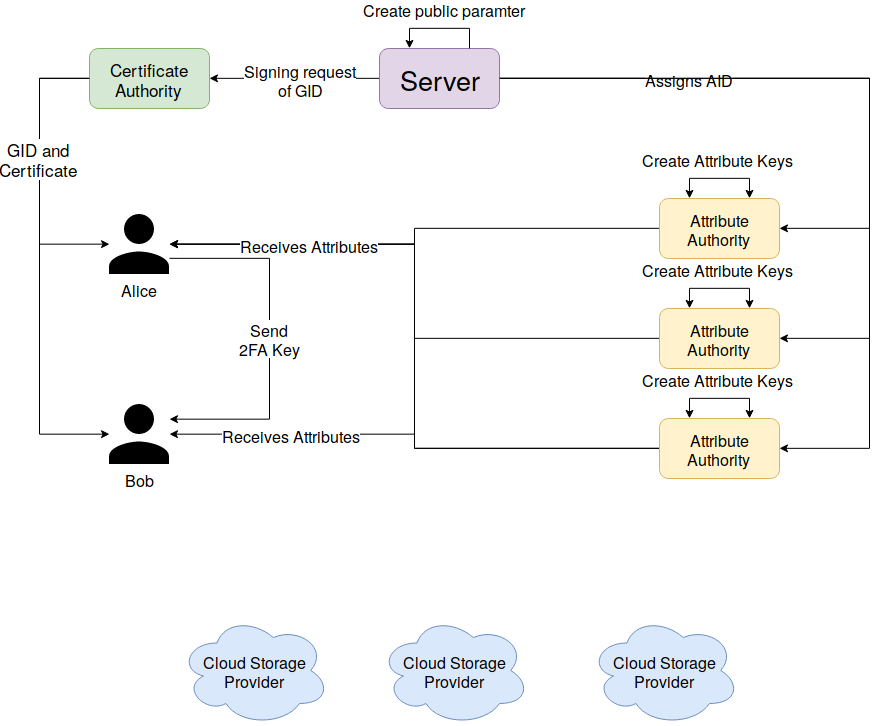
\includegraphics[width=\linewidth]{img/TF-DAC-MACS-overview-setup.png}
    \caption{Setup phase}
    \label{fig:tfdacmacs-setup}
\end{figure}

The setup summarizes the steps of \cite{li2017two} setup, user registration, data owner registration, authority setup, keygen and authentication requests. 

The first step is to create the global public paramters on the server. Thouse paramter are exposed on a public bulliton board and queriable for each entity in this eco system. Since they are required in every step it is assumed that the entity already downloaded this informaiton. 

On AA setup the server frist generates a new AID. This AID will be mapped to the domain name of this entity. So for example the TU-Berlin will have as its ID: "aa.tu-berlin.de". In this way it is ensured that no AID can double. Further, it would be verifable via the certificate chain of TSL/SSL that this AID indeed belongs to the TU-Berlin. To do so the certificate coupled with this domain can be verified and then a query to "aa.tu-berlin.de" would lead to the corresponding AA of the TU-berlin.

The AA is free to generate attribute keys. Attributes also have identifier and values assigned to them. Values and attribute identifier can be any valid string as long as it does not contain any special characters such as ":" or ".". The attribute will have the form of "<AID>.attr.<Attribute\_name>:<Attribute\_value>". For example the major computer sience would be displayed as "aa.tu-berlin.de.attr.major:computer\_sience". Each attribute-value pair gets a secret key assigned. The public component for this attribute will be published on the public bulliton board of the AA. 

In the next step, users are registered to the server. They receive the GID and a certificate for this GID. They can use the certificate later on to register to the AA or to authenticate themself to other users. The GID will have the form "<AID>.user.<UID>" where UID is a universal unique identifier (\ac{UUID}) in version 4.  
User receive their secret attribute keys by retrieving them from their AA. The AA verifies the certificate and issues the user his roles.

In the final setup, users can issue each other two factor keys so called \textit{authentication keys}. This authentication keys introduce a new layer of security where users can decide who exactly can decipher their plaintext. In some cases this may be needed since access policies in ABE describe alsways a group of user. 
If Bob wants to get an authentication key from Alice he sends a authentication request to Alice containing this certificate. Alice checks the validity of the certificate and returns the Bob-specific authentication key.

The previous steps are summarized in the figure \ref{fig:tfdacmacs-setup}.

\subsection{Encryption}
\begin{figure}[!t]
\centering
    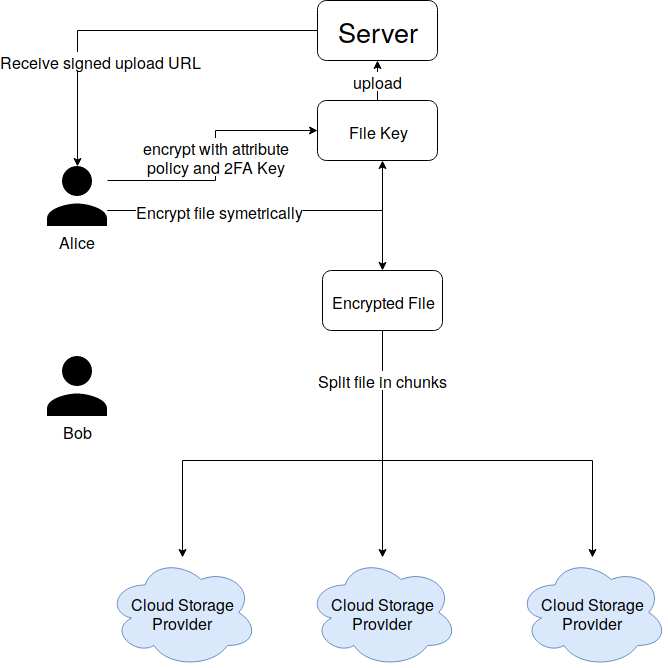
\includegraphics[width=\linewidth]{img/TF-DAC-MACS-overview-encrypt.png}
    \caption{Encryption phase}
    \label{fig:tfdacmacs-encrypt}
\end{figure}

To upload a file encrypted under an access policy Alice first encrypts the file symetrically to create a file key (figure \ref{fig:tfdacmacs-encrypt}). This results in an file key and an encrypted file. The encrypted file is split up into different file chunks. Alice requests from the server a signed upload URL which she can use to upload the chunks to the CSPs. 

The file key, on the other hand, will be encrypted with an access policy defined by Alice. In addition she is also able to encrypt the ciphertext with the authentication key she issued to Bob. This encrypted file key will be uploaded to server where it is stored securly. 

\subsection{Decryption}
\begin{figure}[!t]
\centering
    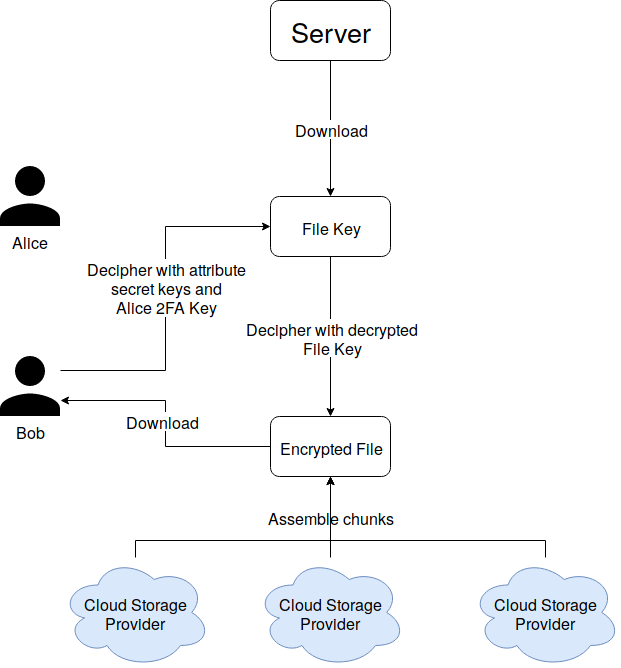
\includegraphics[width=\linewidth]{img/TF-DAC-MACS-overview-decrypt.png}
    \caption{Setup phase}
    \label{fig:tfdacmacs-decryption}
\end{figure}

On decryption first the encrypted file key will be downloaded from the server. If Bob has a matching super set of attributes he can decipher it using his secret attribute keys. He might also apply the two factory key from Alice to endup with the plain file key (figure \ref{fig:tfdacmacs-decryption}. 

Next, he downloads the file chunks from the CSP, assembled them back together and decryphs them with the revocered file key.

\subsection{Revoke attribute}
\begin{figure}[!t]
\centering
    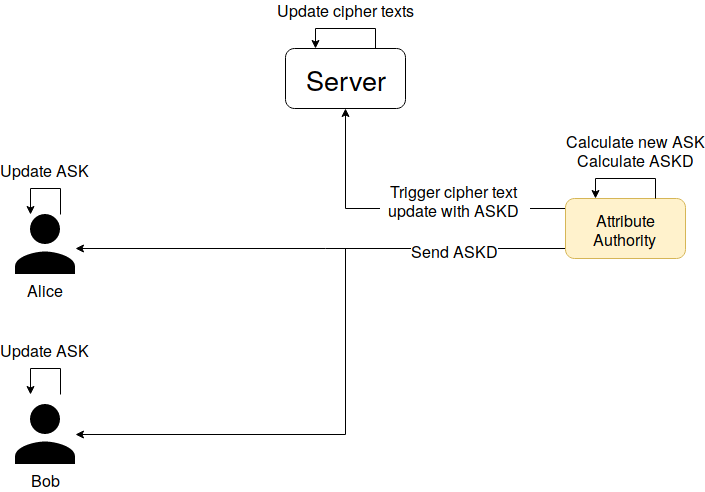
\includegraphics[width=\linewidth]{img/TF-DAC-MACS-overview-revoce-attr.png}
    \caption{Attribute revocation}
    \label{fig:tfdacmacs-attr-revocation}
\end{figure}

As displayed in figure \ref{fig:tfdacmacs-attr-revocation}, a revokation of an attribute key is always triggered by the AA that administers this attriubte. It frist creates a new secret key for the revoked attribute and calculates for each user owning the old attribute a delta. This delta is send to each non revoked user respectivly. In addition, the AA calucates a cipher text update key. This is send to the server which then in turn starts updating all the cipher text for the new attribute secret key. This operation will not affect the plaintext message in any kind. 

Alice and Bob, both receiving their update key, calculate their new attribute secret key. The AA can publish the new attribute public key on its public bulliton board.

\subsection{Revoke two-factor key}
\begin{figure}[!t]
\centering
    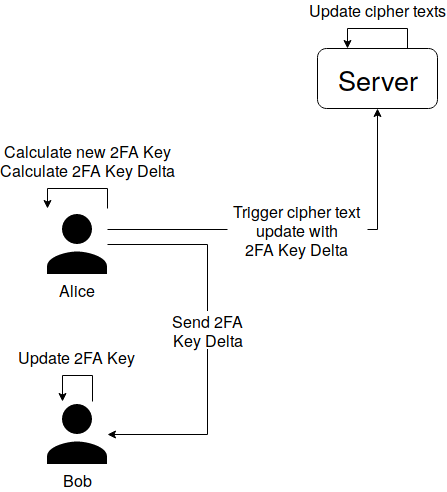
\includegraphics[width=0.6\linewidth]{img/TF-DAC-MACS-overview-revoce-user-key.png}
    \caption{Two-factor key revocation}
    \label{fig:tfdacmacs-user-auth-key-revocation}
\end{figure}

In a similar way as it was done for attribute revocation, Alice now starts to calcuate a new two-factor key. She computes the delta to all old two-factor keys she issed and distributes them to all non-revoced users. Finally, she calculates the ciphertext update key and sends it to the server. The server updates all relevant cipher texts.


\subsection{Adaptions and Improvements}
While TF-DAC-MACS satisfy all the requirementes it fits not perfect. To make the scheme more usable, the fixed two-factor authentication was removed and the key generation of the attribute which was defined in the setup phase as implied that the values need to be known at beginng, was moved to the point where the user requests a new attribute. Further, we propose a simple technique to break up TF-DAC-MACS m-of-n treshold policy with the traidoff for performance. And finally, we a technique proposed in \cite{bethencourt2007ciphertext} to implement numerical values and comparisons in boolean access formular. 

\subsubsection{Removing the fix two-factor contrain}
To make \ac{TF-DAC-MACS} more pratically applicable we removed the fixed two-factor contrain from the encyrption, decryption, and cipher update part. The two factor identifier $\alpha$ is used by the data owner to restirct the access to the content to certain users. 

This leads to the fact that the underlying \ac{ABE} schemes looses some of it expressivness. The zero knowledge of the data owner on which invidual is able to decrypter the cipher text is broken with the two factor part. Here each user that wants to decryper the encrypted text need to make an \textit{authentication request} to the data owner to receive the corresponing decryption key. To restore the possiblity to let an unkown user group decrypter the cipher text, we removed the two factor part. To do so we adapted encryption, decryption and cipher text update. The authentication key update will be ignored since it makes no sense to apply it on a non exisiting authentication key. 

\begin{itemize}
\item \textbf{Encryption:} 
We only need to update the $C_3$ part of the cipher text since it is the only one containing the two factor component $\alpha$.

The original $C_3$:
$$
C_3 = \Big( \prod_{v_{aid_{i}, j}\in W} g^{y_{aid_{i}, j}} \Big)^{s + \alpha} 
$$
is adapted to:
$$
\widehat{C}_3 = \Big( \prod_{v_{aid_{i}, j}\in W} g^{y_{aid_{i}, j}} \Big)^s
$$ 
In addition we will remove $oid$ from the ciphertext describtion since it refferese to the data owner ID. Which is only needed on authentication key update.

\item \textbf{Decryption:}
$SK_W = \prod_{v_{aid_i,j} \in W} SK_{v_{aid_i,j}}$ and $UPK_W = \prod_{v_{aid_i,j} \in W} UPK_{v_{aid_i,j}}$ remain defined in the same was as defined in the paper. 

On decryption the user does not need to generate $UPK_W$ and $SK_{uid, oid}$ anymore. The decryption equation is updated to:

$$
m = \frac{C_1 \cdotp e(H(uid), \widehat{C}_3)}{e(C_2, SK_W)}
$$

Note that the original decryption equation results in the above equation when the two factor part is deducted.

\begin{equation}
\begin{split}
m &= \frac{C_1 \cdotp e(H(uid), C_3)}{e(C_2, SK_W)e(SK_{uid, oid}, UPK_W)} \\
  &= \frac{C_1 \cdotp e\Big(H(uid), \Big( \prod_{v_{aid_{i}, j}\in W} g^{y_{aid_{i}, j}} \Big)^{s + \alpha} \Big)}{e(C_2, SK_W)e(H(uid)^\alpha, \prod_{v_{aid_i,j} \in W} UPK_{v_{aid_i,j}})} \\
  &= \frac{C_1 \cdotp e\Big(H(uid), \Big( \prod_{v_{aid_{i}, j}\in W} g^{y_{aid_{i}, j}} \Big)^{s + \alpha} \Big)}{e(C_2, SK_W)e(H(uid)^\alpha, \prod_{v_{aid_i,j} \in W} g^{y_{aid_i,j}})} \\
  &= \frac{C_1 \cdotp e\Big(H(uid), \Big( \prod_{v_{aid_{i}, j}\in W} g^{y_{aid_{i}, j}} \Big) \Big)^{s + \alpha}}{e(C_2, SK_W)e(H(uid), \prod_{v_{aid_i,j} \in W} g^{y_{aid_i,j}})^\alpha} \\
  &= \frac{C_1 \cdotp e\Big(H(uid), \Big( \prod_{v_{aid_{i}, j}\in W} g^{y_{aid_{i}, j}} \Big) \Big)^{s}}{e(C_2, SK_W)} \\
  &= \frac{C_1 \cdotp e\Big(H(uid), \Big( \prod_{v_{aid_{i}, j}\in W} g^{y_{aid_{i}, j}} \Big)^{s} \Big)}{e(C_2, SK_W)} \\
  &= \frac{C_1 \cdotp e(H(uid), \widehat{C}_3)}{e(C_2, SK_W)}
\end{split}
\label{eq:2faRemoval}
\end{equation}

As shwon, no security is threadned since we end up at the same equation as we would if we had the two factor part included. 

\item \textbf{Attribute revocation:}
The cipher text update key is adapted from

$$
CUK^{ID_W}_{v_{aid_i,j}} = (g^s \cdotp g^\alpha)^{y'_{aid_i,j} - y_{aid_i,j}}
$$

to 

$$
\widehat{CUK}^{ID_W}_{v_{aid_i,j}} = (g^s)^{y'_{aid_i,j} - y_{aid_i,j}}
$$

$\widehat{C}'_3$ now computes as 

\begin{equation}
\begin{split}
\widehat{C}'_3 &= \widehat{C}_3 \cdotp \widehat{CUK}^{ID_W}_{v_{aid_i,j}} \\
&\cdotp \Big( \prod_{v_{aid_{t}, j}\in W, v_{aid_t, j} \neq v_{aid_i,j}} g^{y_{aid_{i}, j}} \Big)^{r} \cdotp (g^{y'_{aid_i,j}})^{r} \\
&= \Big( \prod_{v_{aid_{t}, j}\in W, v_{aid_t, j} \neq v_{aid_i,j}} g^{y_{aid_{i}, j}} \Big)^{s + r} \cdotp (g^{y'_{aid_i,j}})^{s + r}
\end{split}
\end{equation}

It can be shown that $C'_3$ computes to the message $m$ in the same way as shown in eqation \ref{eq:2faRemoval}.

\item \textbf{Authentication update:}
Nothing need to change since cipher text do not contain authentication components. 
\end{itemize}

\subsubsection{Dynamic secret key generation}
Another small tweak in the \ac{TF-DAC-MACS} scheme was that the attributes for each \ac{AA} do not have to be known on AA inizialisation. They can be creates as well on each users key gen. This reduces the universe of possible attribute values to thouse who are actually needed.

\subsection{Extension to m-of-n treshold policy}
Extending to m-of-n treshold policy is also quite straight forward if we are willing to make traide offs in performance. So the client could upload different versions of the plain text encrypted under different policies. A client only need to decipher one of thouse cipher texts to revocer the message.

\subsection{Numerical boolean comparisons}
As described in \cite{bethencourt2007ciphertext} we could display numeric values in binary. Each number $x$ is composed of $\lceil log_2(x) \rceil$ attributes. Each of this attributes relate to either a $1$ or $0$ in one position in the binary number respresentation of $x$. So for example the number $5$ in binary would be displayed as $0101$ and its attribute would be: $x:0***$, $x:*1**$, $x:**0*$ and $x:***1$. 

If a user now wants to create a policy where he challanges a number $x$ to be greater or equal to $3$ he would create a policy: "$(x:1*** or (x:*1** or (x:**1* and x:***1))$". Analogous the policy for $x$ smaller than $4$: "$(x:0*** and (x:*0** or (x:*1** and x:**0* and x:***0))$".

Disadventage of this representation is of cause that it is limited in space. To display a 32-bit number we must issue 64 attriubte values and maintain 64 attriubte value keys. 


\subsection{Technologies}
To develop the first prototype of the system defined previously we will use the following technology stack:

\begin{itemize}
	\item \textbf{Spring boot}
	\item \textbf{Docker}
	\item \textbf{jPBC} \cite{ISCC:DecIov11}
	\item \textbf{...}
\end{itemize}
\todo{write me}

\subsection{Problems}

\subsubsection{En- and decrypting arbitrary data}
TF-DAC-MACS takes as an input for encryption a message $M \in GT$. Since there is not easy way to reconstruct a message from an element in $GT$, we have to combine some encryption teachniques to encrypt arbitrary data. 

The alogirhtm first chooses a random $M \in GT$ and outputs $M$ together with the constructed cipher text. $M$ is then hashed into a byte buffer using \ac{SHA}-256. In the next step we will encrypt our arbitrary data using \ac{AES} and as a key the hash previous computed. 

On decryption we frist reconstruct $M$ using the ABE decryption technique and then hashing $M$ again to reconstruct our AES secret key. This will help us to decipher the data that was encrypted. 

